\documentclass{article}
\usepackage{amsmath}
\usepackage{amssymb}
\usepackage{graphicx}
\usepackage{booktabs}
\usepackage{array}
\usepackage{hyperref}
\usepackage{enumitem}
\usepackage{tikz}
\usetikzlibrary{arrows.meta, positioning}

\title{DSC 257R: Unsupervised Learning \\ Homework 6}
\author{}
\date{}

\begin{document}

\maketitle

\section*{Multivariate Gaussians and Gaussian Processes}

\begin{enumerate}
\item Consider the spherical Gaussian $N(0, I_d)$ in $d$-dimensional space.
    \begin{enumerate}
    \item What is the maximum density achieved by this distribution? At what point is it achieved?
    \item In very rough terms, what happens to the maximum density as $d$ grows? (This helps explain why for high-dimensional data we typically work with the logarithm of the density, in order to avoid numerical underflow errors.)
    \end{enumerate}

\item \textbf{Length concentration.} Write a procedure that draws 10000 points $X_1, \ldots, X_{10000}$ from the spherical Gaussian $N(0, I_d)$ and plots a histogram of their (squared) lengths $\|X_i\|^2$.
    \begin{enumerate}
    \item Do this for $d=10$. What seems to be the typical (squared) length?
    \item Repeat for $d=100$. Is the histogram more concentrated than in (a), or is it less concentrated?
    \end{enumerate}

\item Suppose $X \in \mathbb{R}^2$ has a Gaussian distribution with mean $\begin{bmatrix}1 \\ 2\end{bmatrix}$ and covariance matrix $\begin{bmatrix}2 & 0 \\ 0 & 4\end{bmatrix}$. What is the distribution of the projection of $X$ onto direction $\frac{1}{\sqrt{2}}\begin{bmatrix}1 \\ 1\end{bmatrix}$?

\item We have three sensors $(X_1, X_2, X_3)$ whose joint distribution is Gaussian with mean zero and covariance matrix
    \[
    \begin{bmatrix}
    6 & 3 & 1 \\
    3 & 9 & 0 \\
    1 & 0 & 2
    \end{bmatrix}
    \]
    \begin{enumerate}
    \item What is the distribution of sensor $X_3$?
    \item What is the joint distribution of sensors $X_1, X_2$?
    \item Suppose we observe $X_2=2$ and $X_3=1$. What is the resulting conditional distribution of $X_1$?
    \end{enumerate}

\item \textbf{Modeling temperature data with Gaussian processes.} In this question, we will explore modeling of geospatial data via Gaussian processes. Begin by downloading the files \texttt{gptrain.csv} and \texttt{gptest.csv} from the course webpage. Each row in each file corresponds to a temperature reading at a given weather station in Brazil at 2 pm on January 1, 2021. The first column gives the latitude of the station, the second the longitude, and the final column is the temperature reading in degrees Celsius. We will fit a simple Gaussian Process model on \texttt{gptrain.csv} and use it to infer temperatures at other locations at that same date and time.

We will fit a Gaussian process with covariance function
\[
k(x, x') = \exp\left(\frac{-\|x-x'\|}{\sigma}\right)
\]
and mean function $m(x) = 20$ (degrees Celsius). Here $\|x-x'\|$ denotes Euclidean distance between raw latitude and longitude coordinates.

Denote the locations in \texttt{gptrain.csv} by $X_{\text{tr}}$ and the temperatures at those locations by $y_{\text{tr}}$; define $X_{\text{te}}, y_{\text{te}}$ analogously for \texttt{gptest.csv}. Thus $X_{\text{tr}}$ is a $93 \times 2$ matrix while $y_{\text{tr}}$ is a 93-dimensional vector.

\begin{enumerate}
\item The joint distribution of training and test responses can be written as
    \[
    \begin{bmatrix} y_{\text{tr}} \\ y_{\text{te}} \end{bmatrix} \sim N\left(\begin{bmatrix} 20 \\ \vdots \\ 20 \end{bmatrix}, \begin{bmatrix} K_{\text{tr}} & K_{\text{tr,te}} \\ K_{\text{te,tr}} & K_{\text{te}} \end{bmatrix}\right)
    \]
    where the block matrix
    \[
    \begin{bmatrix} K_{\text{tr}} & K_{\text{tr,te}} \\ K_{\text{te,tr}} & K_{\text{te}} \end{bmatrix}
    \]
    is the matrix arising from all pairwise evaluations of the covariance function $k(\cdot)$ over all training and testing locations, and its diagonal components $K_{\text{tr}}$ and $K_{\text{te}}$ are the matrices arising from all pairwise covariances within the training and test sets, respectively.

    Explain very briefly how the definition of Gaussian process allows us to come to this conclusion.

\item Define
    \[
    m_{\text{te}} := \begin{bmatrix} 20 \\ \vdots \\ 20 \end{bmatrix} \in \mathbb{R}^{11}
    \]
    since there are 11 locations in the test set. Using properties of the Gaussian, it can be shown that the distribution of test responses given training locations, training responses, and test locations, follows
    \[
    y_{\text{te}} \mid y_{\text{tr}}, X_{\text{te}}, X_{\text{tr}} \sim m_{\text{te}} + N\left(K_{\text{te,tr}} \cdot K_{\text{tr}}^{-1}(y_{\text{tr}} - m_{\text{tr}}), K_{\text{te}} - K_{\text{te,tr}} K_{\text{tr}}^{-1} K_{\text{tr,te}}\right)
    \]
    In Bayesian language, this is the posterior predictive distribution.

    \begin{itemize}
    \item Using $X_{\text{tr}}, X_{\text{te}}$, and $y_{\text{tr}}$, compute the posterior mean of $y_{\text{te}}$ via matrix multiplication, using $\sigma=1.5$ in the covariance function. Report the mean squared error between your computed posterior mean and the true values found in $y_{\text{te}}$.
    \item Report the mean squared error that you would have obtained by simply predicting the average value in $y_{\text{tr}}$ for all locations.
    \end{itemize}

\item The diagonal of the posterior predictive matrix
    \[
    K_{\text{te}} - K_{\text{te,tr}} K_{\text{tr}}^{-1} K_{\text{tr,te}}
    \]
    gives the conditional variances of the test responses given $X_{\text{tr}}, X_{\text{te}}$, and $y_{\text{tr}}$.

    \begin{itemize}
    \item Create a rich grid (at least 5000 points) of test latitudes and longitudes within the range found in the training set. Make a plot showing the predicted (posterior mean) temperature at all points in the grid. You might find the function \texttt{matplotlib.pyplot.imshow} helpful for this.
    \item Make another plot showing the standard deviation of the prediction at all points in the grid. Plot the locations of the stations found in the training set as well.
    \item What do you notice about the relationship of the standard deviation of the prediction and the distance of that prediction to a training point?
    \end{itemize}
\end{enumerate}
\end{enumerate} % Close the enumerate environment for the first section

\section*{Bayes Nets and Autoregressive Models}

\begin{enumerate} % Start a new enumerate environment for the second section
\addtocounter{enumi}{5} % Continue numbering from where we left off

\item \textbf{Four friends} $F_1, F_2, F_3, F_4$ like going to the movies. When a new movie comes out, they behave according to the following scheme:
    \begin{itemize}
    \item $F_1$ sees the movie with probability 0.5.
    \item $F_2$ sees the movie with probability 0.7, independently.
    \item If either of $F_1$ or $F_2$ (or both) see the movie, $F_3$ goes to see it with probability 0.8; if neither $F_1$ nor $F_2$ sees the movie, $F_3$ sees it with probability 0.3.
    \item If $F_3$ sees the movie, then $F_4$ goes to see it with probability 0.9. If $F_3$ doesn't see the movie, then $F_4$ sees it with probability 0.5.
    \end{itemize}

    Let $F_1, F_2, F_3, F_4 \in \{0,1\}$ denote who sees the movie. The dependencies between these four random variables can be captured by the following directed graph:

    \begin{center}
    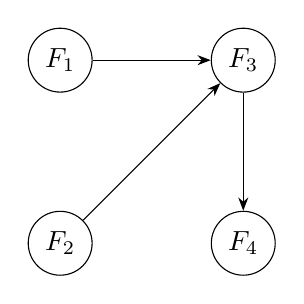
\begin{tikzpicture}[node distance=1.5cm]
        \node[circle, draw] (F1) {$F_1$};
        \node[circle, draw, below=of F1] (F2) {$F_2$};
        \node[circle, draw, right=of F1] (F3) {$F_3$};
        \node[circle, draw, below=of F3] (F4) {$F_4$};

        \draw[-Stealth] (F1) -- (F3);
        \draw[-Stealth] (F2) -- (F3);
        \draw[-Stealth] (F3) -- (F4);
    \end{tikzpicture}
    \end{center}

    \begin{enumerate}
    \item Give the conditional probability tables for this Bayes net.
    \item What is the probability of the configuration $F_1 = F_2 = F_3 = 1, F_4 = 0$?
    \end{enumerate}

\item \textbf{Non-uniqueness of underlying DAG.} Suppose random variables $X$ and $Y$ take values in $\{0,1\}$. Does the joint distribution of $(X, Y)$ necessarily factor over the DAG on the left below? What about the DAG on the right?

    \begin{center}
    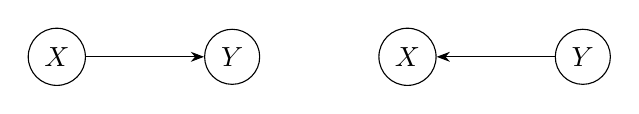
\begin{tikzpicture}[node distance=1.5cm]
        \node[circle, draw] (F1) {$X$};
        \node[circle, draw, right=of F1] (F3) {$Y$};
        \node[circle, draw, right=of F3] (F2) {$X$};
        \node[circle, draw, right=of F2] (F4) {$Y$};
        \draw[-Stealth] (F1) -- (F3);
        \draw[-Stealth] (F4) -- (F2);
    \end{tikzpicture}
    \end{center}

\item \textbf{Genes, diseases, and outcomes.} There is a fictitious disease $(D)$ that can cause paralysis $(P)$. Whether or not an individual gets this disease depends in large part on two genes, $G_1$ and $G_2$. Here is a summary:

    \begin{itemize}
    \item Each of these genes $G_1, G_2$ can either be normal (also known as wild-type), represented by $G_i=0$, or mutant, represented by $G_i=1$.
    \item For a person with $G_1=G_2=0$ (both genes wild-type) the probability of acquiring the disease is zero. If $G_1$ is mutant and $G_2$ is wild-type, the probability is 0.2. If $G_1$ is wild-type and $G_2$ is mutant, it is 0.1. And if both genes are mutant, then the disease probability is 0.5.
    \item For an individual with the disease, the probability of paralysis is 0.5. Without the disease, there is still a small probability of paralysis (from other causes): 0.01.
    \item $G_1$ is mutant with probability 0.1 and $G_2$ is mutant with probability 0.2; these are independent.
    \end{itemize}

    \begin{enumerate}
    \item Draw a suitable Bayes net over the variables $G_1, G_2, D, P$, and give all relevant conditional probability tables. Let $D=1$ if the disease is present and $D=0$ if it isn't; likewise with paralysis.
    \item What is the probability of disease $(D=1)$?
    \item What is the probability of paralysis $(P=1)$?
    \item We observe that a person has paralysis. What is the probability that they have the disease?
    \item We observe that a person has the disease $(D=1)$. What is the probability that they have the mutant form of gene $G_1$?
    \end{enumerate}

\item \textbf{A character-level RNN for text generation.} Download the file \texttt{rnn-gen.zip} from the course webpage; it contains a Jupyter notebook saved as .py, \texttt{text-gen-rnn.ipynb}, as well as data and helper files. The notebook is adapted from an excellent blog post by Andrej Karpathy, \textit{The unreasonable effectiveness of recurrent neural networks}. It fits an RNN (more precisely, an LSTM) to the text of Shakespeare's plays and then uses this to generate more text, one character at a time.

Work through the notebook and try to understand what is going on. There are just three small questions to answer.

\begin{enumerate}
\item How many characters are we considering, and what is the integer code for 'A'?
\item What is the length of the corpus in characters?
\item The input and output size for the RNN are set to 66. Why is this?
\end{enumerate}
\end{enumerate}

\end{document}
